\listfiles
\documentclass[twoside,12pt]{article}
\newcommand{\dataset}{{\cal D}}
\newcommand{\fracpartial}[2]{\frac{\partial #1}{\partial  #2}}
\usepackage{hyperref}
\usepackage{enumerate}
\usepackage[top=2in, bottom=1.5in, left=0.85in, right=0.5in]{geometry}
\usepackage[hyphenbreaks]{breakurl}
%\usepackage[pdfstartview=FitH,pdfstartpage=13,pdfpagemode=UseNone]{hyperref}
\usepackage{amsfonts}
\usepackage{graphicx} 
\usepackage[linesnumbered,ruled]{algorithm2e}
\usepackage{float}
\usepackage{amssymb,amsmath}
\usepackage{mdwlist }
\usepackage{color}
\usepackage{multirow}
\usepackage{listings}
\usepackage{float}
\usepackage{setspace}
\usepackage[english]{babel}

\usepackage{graphicx}
\usepackage{caption}
\usepackage{subcaption}


\definecolor{darkblue}{rgb}{0.0,0.0,0.5}
\newtheorem{Dfn}{Definition}
\hypersetup{colorlinks,breaklinks,
            linkcolor=darkblue,urlcolor=darkblue,
            anchorcolor=darkblue,citecolor=darkblue}
\newcommand{\sign}{\text{sign}}
\newcommand{\argmin}{\arg\!\max}
\begin{document}

\title{Recursive Auto Encoder (RAE)
Method of Learning Meanings for Sentences\\  Learning Algorithms, Project 4}
\author{Mohsen Malmir, Erfan Sayyari}
\maketitle

\section{Abstract}

\section{Introduction}

\section{Design and Analysis of Algorithm}

\subsection{Recursive definition of meaning}
In the context of deep learning to represent the semantic content of sentences, we need to represent each word by a vector, and then represent their relative relation by a tree. We use binary tree representation and each word is a leaf node of the tree, and there are $n-1$ internal nodes, where $n$ is the length of the sentence. Each of the internal nodes shows the phrase of two or more consecutive words. To represent the meaning of each node we use a vector of $\mathbb{R}^d$.

We use a random initialization to represent the meaning of each node in $\mathbb{R}^d$. Each random vector is produced from a Gaussian of dimension $d$ with zero mean and diagonal covariance matrix $\sigma^2I$ independent from each other. 

To obtain the meaning of each internal node (say node $k$), rather than leaf nodes, we use the following equation:
\begin{equation}
x_k=h(W[x_i;x_j]+b)
\end{equation}
where $i$ and $j$ are children of node $k$, and $W$ is a matrix in $\mathbb{R}^{d\times2d}$ and $b$ is a vector in $mathbb{R}^d$. The function $h$ is a pointwise sigmoid-shaped function from $\mathbb{R}^d$ to the interval $[-1,+1]^d$.

In the training stage, we need to learn parameters $W$ and $b$. Since our problem is a supervised method, we need a target value for the meaning of the sentences. We use the notation $x_r$ to represent the predicted meaning of the sentence (of the root node r). If the true target value of the sentence is $t$, the loss function could be for example $E=(t-x_r)^2$, and for training we need to minimize this error. To do minimization we need to compute $\frac{\partial{E}}{\partial{W}}$ and $\frac{\partial{E}}{\partial{b}}$ and use a stochastic gradient descent (SGD) algorithm to minimize $E$ for the all of sentences, or we can use LBFGS quasi-Newton method.  
\subsection{Autoencoders}
In the autoencoder approach, we want to change the goal of supervised learning to find the parameters $W$, $b$ automatically without training labels provided from the outside. We could consider the meaning of the node $x_k$ is equal to:
\begin{equation}
x_k=h(W[x_i;x_j]+b).
\end{equation}

We represent two other variables, $z_i$ and $z_j$ such that:
\begin{equation}
[z_i;z_j]=Ux_k+c
\end{equation}
where $U$ is a matrix in $\mathbb{R}^{2d\times d}$ and $c$ is a vector in $\mathbb{R}^{2d}$, where $z_i$ and $z_j$ are approximation reconstructions of the inputs $x_i$ and $x_j$, and $U$ and $c$ are additional parameters. So we can define a new loss as:
\begin{equation}
E=||x_i-z_i||^2+||x_j-z_j||^2=||[x_i;x_j]-Uh(W[x_i;x_j]+b)-c||^2.
\end{equation}

For the whole sentence the error is the sum of error of reconstruction of all non-leaf nodes. So we can use this reconstruction error to learn $W$, $b$, $U$, and $c$ with no training labels provided from the outside. 

This approach has two other refinements. In order not to train the system to the trivial solution which leads to zero error we need to justify the equations. The trivial solution is all the parameters equal to zero. So the error will be zero. In order to solve it we can normalize the equation for the meaning of $k^th$ node such that:
\begin{equation}
x_k = \frac{h(W[x_i;x_j]+b}{||h(W[x_i;x_j]+b||}.
\end{equation}
This leads the $h$ function not to be pointwise anymore, and derivatives are much harder in this case.

The other refinement is based on the intuition that the error of reconstruction of the longer phrases are much more important. Therefore, the definition of the loss for node $k$ is equal to:
\begin{equation}
E_1(k)=\frac{n_i}{n_i+n_j}||x_i-z_i||^2+\frac{n_j}{n_i+n_j}||x_j-z_j||^2
\end{equation}
where $z_i$ and $z_j$ are as before, and $n_i$ and $n_j$ are how many words are covered by nodes $i$ and $j$.
\subsection{ Selecting a tree structure}
After training the parameters automatically, we will generate a method to reconstruct the tree automatically as well. For a given sentence, if $T$ be the set of non-leaf nodes of its binary tree, the error of the whole tree is equal to:
\begin{equation}
\sum_{k \in T}E_1(k).
\end{equation}

For a sentence of length $n$, there is a finite number of possible trees calculated from the Catalan number of $C_{n-1}$, where $C_n$ is:
\begin{equation}
C_n= {2n \choose n} -{ 2n\choose n+1}.
\end{equation}
We can define an optimal tree to be the one that minimizes the total error. This optimal tree can be found by the exhaustive search or we can find it by a greedy algorithm approximately. 

The greedy algorithm is as follows: first, we consider all $n-1$ pairs of neighboring words. Then we find the best pair based on reconstruction error with smallest error. Now omit their combination, and find the best pair based on remaining pairs. 

A small change in the parameter values either causes no change in the optimal tree obtained by greedy algorithm or a jump to a different tree. Generally, gradient descent could cause cycling between two or more different trees, without convergence, while LBFGS would converge smoothly.

\begin{algorithm}[h!]
\# Input: Training Examples $<x_1, x_2, \ldots, x_n>$\\ 
\# Output: Optimal Tree T\\
Nodes=$\{x_1,x_2,\ldots,x_n\}$\\
\While{$Nodes.remaining>1$}{
$MinErrorFound = \inf$\\
$j=-1$\\
ConcatenatingNode = $null$\\
\For{from $i=1$ to $i=Nodes.remaining-1$}{
Compute $p\leftarrow h(W^{(1)}[c_1;c_2]+b^{(1)})$\\
Compute $[\hat{c}_1;\hat{c}_2] \leftarrow W^{(2)}p+b^{2}$\\
$Error \leftarrow E_1([c_1;c_2],[\hat{c}_1;\hat{c}_2])$\\
\If{$Error<MinErrorFound$}{
MinErrorFound $\leftarrow$ $Error$\\
$j \leftarrow i$
ConcatenatingNode $\leftarrow p$
}
}
ConcatenatingNode.leftChild $\leftarrow$ $Nodes(j)$\\
ConcatenatingNode.rightChild $\leftarrow$ $Nodes(j+1)$\\
Nodes $\leftarrow Nodes-\{Nodes(j), Nodes(j+1)\}+\{ConcatenatingNode\}$
}
$T.root$ $\leftarrow$ ConcatenatingNode
\caption{Constructing the Tree using Greedy Algorithm}
\label{algorithm tree}
\end{algorithm}
 
\subsection{Using meaning to predict labels}
We can have a target value rather than target meaning for a sentence to be predicted. For example, positivity or negativity of the sentence, which is binary. 

Each node of the tree (say node $k$) has a meaning vector $x_k$, and we can add a linear model to each node to predict target value of each node. If the values of the predicted labels are binary, then linear model is a standard logistic regression classifier, and if there are more than two classes, the model is multinomial or multiclass logistic regression.

Suppose that we have $r$ different discrete labels and $x_k$ be the meaning of node $k$. Then the vector of predicted probabilities of the label values is equal to:
\begin{equation}
\bar{p}=softmax(Vx_k)
\end{equation}
where $V$ is a matrix in $\mathbb{R}^{r\times d}$. If we have $\bar{t}$ to be the true binary vector of length $r$ of node $k$, then we can define squared error of the prediction as $||\bar{t}-\bar{p}||^2$, or we can define log loss as:
\begin{equation}
E_2(k)=-\sum_{i=1}^{r}t_i\log{p_i}.
\end{equation}
We predict the target values for all the internal nodes except leaf nodes. 

If we consider a collection $S$ of $m$ labeled training sentences, then we could write the loss function as:
\begin{equation}
J=\frac{1}{m}\sum_{<s,t> \in S}E(s,t,\theta)+\frac{\lambda}{2}||\theta||^2
\end{equation}
where $\theta=<W,b,U,c,V>$ is all the parameters of the model, and $\lambda$ is a regularization factor, and $E(s,t,\theta)$ is the total error for one sentence $s$ with label $t$ which is equal to:
\begin{equation}
E(s,t,\theta)=\sum_{k \in T(s)}\alpha E_1(k)+(1-\alpha)E_2(k)
\end{equation}
where $T(s)$ is the set of non-leaf nodes of the tree is constructed by the greedy algorithm for the sentence $s$. 

In order to update the meaning of a node $x_n$, we can compute the derivative of the loss with respect to $x_n$ and update it. More particularly, to do this task we use the error of label targets $E_2$. We can write the general equation as:
\begin{equation}
\frac{\partial}{\partial x_n}\sum_{<s,t>\in S}\sum_{k \in T(s)}E_2(k).
\end{equation}
\subsection{Back-propagation for vector-valued nodes}
The complete loss function $J$ is consisted of error of reconstruction $E_{rec}$ or $E_1$ and error of prediction $E_2$:
\begin{align}
J=\frac{1}{N}\sum_{s,t}E(s,t;\theta)+\frac{\lambda}{2}||\theta||^2\\
=\sum_{k \in T(s)}\alpha E_1(k)+(1-\alpha)E_2(k)+\frac{\lambda}{2}||\theta||^2
\end{align}
where $\theta=<W^{(1)},b^{(1)},W^{(2)},b^{(2)},W^{(label)},Leaves>$. As we calculate, the partial derivative of the loss function $J$ with respect to parameters $\theta$ is equal to:
\begin{equation}
\frac{\partial J}{\partial \theta}=\frac{1}{N}\sum_{s,t}\frac{\partial E(s,t;\theta)}{\partial \theta}+\lambda \theta
\end{equation}

We have different activation and values in the network:
\begin{equation}
p=h(a)=h([W^{(1)} b^{(1)}][c_1;c_2;1])
\end{equation}
\begin{equation}
e=[\hat{c}_1;\hat{c}_2]=[W^{(2)} b^{(2)}][p;1]
\end{equation}

\begin{equation}
r = softmax(a^{output})=softmax([W^{label} b^{label}][p_r;1])
\end{equation}
where $r$ is a vector in $\mathbb{R}^q$ (the number of classes is $q$), and $r$ is the predicted probabilities for the classes. Here $p_r$ is the meaning vector for the output node, and $W^{label}$ is a matrix in $\mathbb{R}^{q\times d}$.

We can concatenate $W^{(1)}$ with $b^{(1)}$ and we can concatenate $W^{(2)}$ with $b^{(2)}$:
\begin{equation}
W^{(1*)}=[W^{(1)} b^{(1)}]
\end{equation}
\begin{equation}
W^{(2*)}=[W^{(2)} b^{(2)}]
\end{equation}

Softmax is not a point-wise function, and $r_j$ is equal to:

\begin{equation}
r_j=f_j((W^{label}p_r)_1,(W^{label}p_r)_2,\ldots,(W^{label}p_r)_q)=\frac{e^{(W^{label}p_r)_j}}{\sum_{i=1}^{q}e^{(W^{label}p_r)_j}}
\end{equation}

\begin{equation}
r =
\begin{pmatrix}
  f_1(\sum_{j=1}^{d}W^{label}_{1j} p_{r_j}, \sum_{j=1}^{d}W^{label}_{2j}p_{r_j},\ldots, \sum_{j=1}^{d}W^{label}_{qj}p_{r_j})\\
   f_2(\sum_{j=1}^{d}W^{label}_{1j}p_{r_j}, \sum_{j=1}^{d}W^{label}_{2j}p_{r_j},\ldots, \sum_{j=1}^{d}W^{label}_{qj}p_{r_j}) \\
  \vdots  \\
    f_q(\sum_{j=1}^{d}W^{label}_{1j}p_{r_j}, \sum_{j=1}^{d}W^{label}_{2j}p_{r_j},\ldots, \sum_{j=1}^{d}W^{label}_{qj}p_{r_j})\\
 \end{pmatrix}
\end{equation}
 So we could consider $a^{output}=W^{label}p_r$ as, which is a vector in $\mathbb{R}^q$ and rewrite the r as:
 \begin{equation}
 r=
 \begin{pmatrix}
 f_1(a^{output}_1,a^{output}_2,\ldots,a^{output}_q)\\
  f_2(a^{output}_1,a^{output}_2,\ldots,a^{output}_q)\\
\vdots \\
 f_q(a^{output}_1,a^{output}_2,\ldots,a^{output}_q)\\
 \end{pmatrix}
\end{equation}
Now, we want $\frac{\partial J}{\partial W^{(1)}_{i,j}}$, which is not explicitly related to loss function $J$. We could write:
\begin{equation}
p_r=h(W^{(1)}[c_1;c_2]+b^{(1)}])
\end{equation} 
where $h$ is a pointwise highly nonlinear function. Now we could have:

We need the partial derivatives of the loss function with respect to parameters:
\begin{equation}
\frac{\partial J}{\partial W^{(1*)}_{ij}} = \frac{\partial J}{\partial a_i}\frac{\partial a_i}{\partial W^{(1*)}_{ij}}=\delta_i \frac{\partial a_i}{\partial W^{(1*)}_{ij}}
\end{equation}
\begin{equation}
\frac{\partial a_i}{\partial W^{(1*)}_i}=[c_1;c_2;1]^T
\end{equation}
\begin{equation}
\frac{\partial J}{\partial W^{(2*)}_{ij}} = \frac{\partial J}{\partial e_i}\frac{\partial e_i}{\partial W^{(2*)}_{ij}}=\gamma_i \frac{\partial e_i}{\partial W^{(2*)}_{ij}}
\end{equation}
\begin{equation}
\frac{\partial e_i}{\partial W^{(2*)}_i}=[x_p;1]^T
\end{equation}
\begin{equation}
\frac{\partial J}{\partial W^{label}_{ij}} = \frac{\partial J}{\partial a^{output}_i}\frac{\partial a^{output}_i}{\partial W^{label}_{ij}}=\zeta_i \frac{\partial a^{output}_i}{\partial W^{label}_{ij}}
\end{equation}
\begin{equation}
\frac{\partial a^{output}_i}{\partial W^{label}}=[x_r;1]^T
\end{equation}

We want to calculate $\gamma_i$ which just related to error of reconstruction, $E_1$:
\begin{equation}
\gamma_i=\frac{\partial J}{\partial e_i} = \alpha\frac{n_1}{n_1+n_2}2(c_1-\hat{c}_1)^T(-\frac{\partial \hat{c}_1}{\partial e_i})+\alpha\frac{n_2}{n_1+n_2}2(c_2-\hat{c}_2)^T(-\frac{\partial \hat{c}_2}{\partial e_i})
\end{equation}
\begin{equation}
\frac{\partial [\hat{c}_1;\hat{c}_2]}{\partial e_i}=1
\end{equation}
\begin{equation}
\gamma_i=-\alpha[\frac{n_1}{n_1+n_2}2(c_1-\hat{c}_1);\frac{n_2}{n_1+n_2}2(c_2-\hat{c}_2)]
\end{equation}
where $\delta_i=\frac{\partial J}{\partial a^{(r)}_i}$ contains all nonlinearity. Now we could write:
\begin{equation}
\frac{\partial J}{\partial a^{(r)}_i}= \sum_{k=1}^q\frac{\partial J}{\partial r_k}\frac{\partial r_k}{\partial a^{(r)}_i}
\end{equation}
$\frac{\partial J}{\partial r_k}=\frac{-t_k}{r_k}$, and we want $\frac{\partial r_k}{\partial a^{(r)}_i}$:
\begin{equation}
\frac{\partial r_k}{\partial a^{(r)}_i}=\frac{\partial f_k}{\partial a^{(r)}_i}=\sum_{t=1}^{q}\frac{\partial f_k}{\partial a^{output}_{t}}\frac{\partial a^{output}_t}{\partial a^{(r)}_i}
\end{equation}

The output node with values $r$, the contribution to J is with the error of classification $E_2$.

\begin{equation}
\zeta_i=\frac{\partial J}{\partial a^{output}_i}=(1-\alpha)\frac{\partial }{\partial a^{output}_i}\sum_{l=1}{q}t_l\log{r_l}
\end{equation}
If $l=k$:
\begin{equation}
\frac{\partial f_i}{\partial a^{output}_{i}}=r_i(1-r_i)
\end{equation}
and if $l\neq i$
\begin{equation}
\frac{\partial f_i}{\partial a^{output}_{l}}=-r_ir_l
\end{equation}
So we could calculate $\zeta_i$ as:
\begin{equation}
\zeta_i = -(1-\alpha)\sum_{l,l\neq i}^q\frac{t_i}{r_i}(-r_lr_i)-(1-\alpha)\frac{r_i}{1-r_i}=(1-\alpha)(r_i-t_i)
\end{equation}

For the internal values $p$, they contribute to loss $J$ through the $[\hat{c}_1;\hat{c}_2]$, $r$:

\begin{align}
\delta_i=\frac{\partial J}{\partial a_i}=\sum_{k=1}^{d}\frac{\partial J}{\partial a_k}\frac{\partial a_k}{\partial a_i}+\sum_{k=1}^{2d}\frac{\partial J}{\partial e_k}\frac{\partial e_k}{\partial a_i}+\sum_{k=1}^{q}\frac{\partial J}{\partial a^{output}_k}\frac{\partial a^{output}_k}{\partial a_i} \\
= \sum_{k=1}^{d}\delta_k\frac{\partial a_k}{\partial a_i}+\sum_{k=1}^{2d}\gamma_k\frac{\partial e_k}{\partial a_i}+\sum_{k=1}^{q}\zeta_k\frac{\partial a^{output}_k}{\partial a_i}
\end{align}
Now we need to compute $\frac{\partial a_k}{\partial a_i}$, $\frac{\partial a^{output}_k}{\partial a_i}$, and $\frac{\partial e_k}{\partial a_i}$:
\begin{equation}
\frac{\partial a_k}{\partial a_i}=\frac{\partial}{\partial a_i}[W^{(1*)}[\ldots;h(a);\ldots;1]]_k=V_{ki}h'(a_i)
\end{equation}
where $V_{ki}$ is the part of $W^{(1*)}$ that multiplies a.

\begin{equation}
\frac{\partial e_k}{\partial a_i}=\frac{\partial}{\partial a_i}[W^{(2*)}[h(a);1]]_k = W^{(2*)}_{ki}h'(a)
\end{equation}
\begin{equation}
\frac{\partial a^{output}_k}{\partial a_i}=\frac{\partial }{\partial a_i}[W^{label}[h(a);1]]_k=W^{label}_{ki}h'(a)
\end{equation}
\begin{align}
\delta_i=\sum_{k=1}^{d}\delta_kV_{ki}h'(a_i)+\sum_{k=1}^{2d}\gamma_kW^{(2*)}_{ki}h'(a_i)+\sum_{k=1}^q \zeta_k W^{label}_{ki}h'(a_i)\\
=h'(a_i)(\sum_{k=1}^{d}\delta_kV_{ki}+\sum_{k=1}^{2d}\gamma_kW^{(2*)}_{ki}+\sum_{k=1}^q \zeta_k W^{label}_{ki})
\end{align}

For the leaves we could write:
\begin{equation}
\frac{\partial J}{\partial x_i}=\delta_{x_i
}\end{equation}


\subsection{Calculating derivatives for normalized vectors}
We derive the above equation for unnormalized vectors. For the normalized vectors and function we have:
\begin{equation}
h(a)=\frac{\tanh(a)}{||\tanh(a)||}
\end{equation}
\begin{equation}
h'(a)=
\begin{bmatrix}
sech^2(a_1) & \ldots & 0 \\
\vdots & \ddots & \vdots \\
0 & \ldots & sech^2(a_d) \\
\end{bmatrix} \times 
\begin{bmatrix}
\frac{1}{||tanh(a)||}I-\frac{1}{||tanh(a)||^3}tanh(a)tanh(a)^T
\end{bmatrix}
\end{equation}
\subsection{Summarizing Derivatives}
for the output nodes $\hat{c}_1$, $\hat{c}_2$, and $r$:
\begin{equation}
\gamma = \frac{\partial J}{\partial e} = 
\begin{bmatrix}
-2\alpha\frac{n_1}{n_1+n_2}(c_1-\hat{c}_1);-2\alpha\frac{n_2}{n_1+n_2}(c_2-\hat{c}_2)
\end{bmatrix}
\end{equation}
\begin{equation}
\zeta = \frac{\partial J}{\partial a^{output}} = 
(1-\alpha)(r-t)
\end{equation}
For the internal nodes,$p$ we have:
\begin{equation}
\delta = h'(a).
\begin{bmatrix}
W^{{(1*)}^T}\delta_q+W^{{(2*)}^T}\gamma+W^{{(label)}^T}\zeta+\frac{\partial E_rec(p,\hat{p})}{\partial p}
\end{bmatrix}
\end{equation}

For the leaf nodes, $x$ we have:
\begin{equation}
\delta_x=
\begin{bmatrix}
W^{{(1*)}^T}\delta_q+W^{{(label)}^T}\zeta+\frac{\partial E_rec(x,\hat{x})}{\partial x}
\end{bmatrix}
\end{equation}
So the derivatives for the parameters are equal to:
\begin{equation}
\frac{\partial J}{\partial W^{(1*)}}=\delta[c_1;c_2;1]^T
\end{equation}
\begin{equation}
\frac{\partial J}{\partial W^{(2*)}}=\delta[p;1]^T
\end{equation}
\begin{equation}
\frac{\partial J}{\partial W^{(label)}}=\delta[p;1]^T
\end{equation}

We could calculate the numerical gradients using the following equation and then compare it with our results above:
\begin{equation}
\frac{\partial J}{\partial \theta}=\frac{J(\theta+\epsilon)-J(\theta-\epsilon)}{2\epsilon}+O(\epsilon^2)
\end{equation}
\begin{algorithm}[h!]
\# Input: Training Examples $<x_1, x_2, \ldots, x_n>$\\ 
\# Output: Training Model\\$\theta=<W^{(1)},b^{(1)},W^{(2)},b^{(2)},W^{label},Leaves>$\\ 
\#Initialization
Initialize word meaning vectors $x_i \sim \mathcal{N}(0,\sigma^2)$\\
Initialize matrices $W^{(1)}$, $W^{(2)}$, $W^{label}, b^{1},b^{2}$ randomly.\\
\While{Not Converged or Exceeds the Maximum Number of Iteration}{
Initialize Gradient $\bigtriangledown J \leftarrow 0$
\For{all $x_i$ }{
Compute $Tree=RAE_{\theta}(x_i)$	\\
	Compute Gradient  $\bigtriangledown J_i \leftarrow \frac{\partial J(x_i)}{\partial \theta}$\\
	Update Total Gradient $\bigtriangledown J \leftarrow \bigtriangledown J + \bigtriangledown J_i$
	}
Update $\theta$ $ \leftarrow$ $\frac{1}{N}$ $\bigtriangledown$ $J+\lambda \theta$}
\caption{Training the Recursive Autoencoder}
\label{algorithm RA}
\end{algorithm}


\section{Design of Experiment}
In this section, we perform a series of experiments to validate the proposed model. First, we perform test to validate the correctness of derivatives calculated in the previous section. We use the numerical gradients calculated using the following equation as the reference,
\begin{equation}
\frac{\partial J}{\partial \theta}=\frac{J(\theta+\epsilon)-J(\theta-\epsilon)}{2\epsilon}+O(\epsilon^2).
\end{equation}
We perform 4 series of experiments. The first two are with softmax classification function and normalized vectors, one with leaf update and the other without leaf update. The second two experiments are the same with tanh classification function. For each experiment, we show the norm of gradient as a sign of convergence of the algorithm. The recognition rate of the model for each approach is demonstrated on the test set, which is $1/3$ of the movie review dataset. This is a dataset containing 10662 movie reviews, equally distributed between two different positive and negative classes. And finally, we show the most positive and negative words learned for the version where the leaves are updated.

\section{Results}
\subsection{Gradient Check}
Figure \ref{figGradCheck} shows the absolute value of the difference between numerical and gradients we derived in this paper. This figure shows the absolute difference value as a function of $\epsilon$ for softmax and tanh network. It is obvious that the derivatives are correct in comparison to the numerical derivatives.

\begin{figure}
\centering
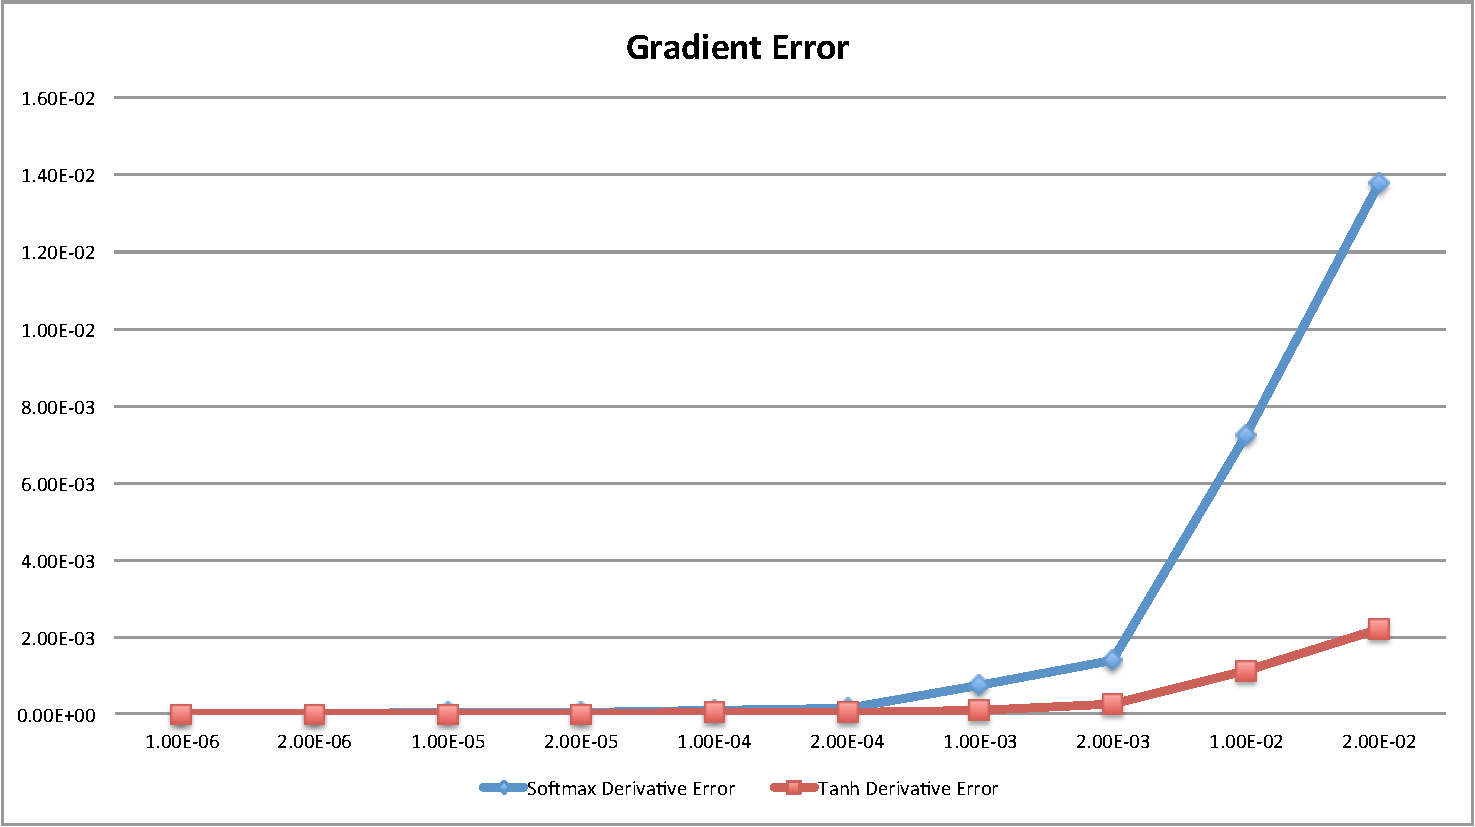
\includegraphics[width=1.\textwidth]{gradError.pdf}
\caption{Absolute difference between the numerical gradient and derivatives we derived in this paper.}
\label{figGradCheck}
\end{figure}

\subsection{Convergence of Model Training}


\subsection{Recongition Performance on Test Set}
To further test the 

\section{Discussion}



\begin{thebibliography}{9}
\bibitem{fastlda}
Porteous, Ian, et al. "Fast collapsed gibbs sampling for latent dirichlet allocation." Proceedings of the 14th ACM SIGKDD international conference on Knowledge discovery and data mining. ACM, 2008.


\bibitem{harmonic}
Newton, Michael A., and Adrian E. Raftery. "Approximate Bayesian inference with the weighted likelihood bootstrap." Journal of the Royal Statistical Society. Series B (Methodological) (1994): 3-48.
APA	

\bibitem{wallach}
Wallach, Hanna M., et al. "Evaluation methods for topic models." Proceedings of the 26th Annual International Conference on Machine Learning. ACM, 2009.

\end{thebibliography}




\end{document}
